\documentclass[pdf,9pt,xcolor=dvipsnames,hide notes]{beamer}\usepackage[]{graphicx}\usepackage[]{color}
%% maxwidth is the original width if it is less than linewidth
%% otherwise use linewidth (to make sure the graphics do not exceed the margin)
\makeatletter
\def\maxwidth{ %
  \ifdim\Gin@nat@width>\linewidth
    \linewidth
  \else
    \Gin@nat@width
  \fi
}
\makeatother

\definecolor{fgcolor}{rgb}{0.345, 0.345, 0.345}
\newcommand{\hlnum}[1]{\textcolor[rgb]{0.686,0.059,0.569}{#1}}%
\newcommand{\hlstr}[1]{\textcolor[rgb]{0.192,0.494,0.8}{#1}}%
\newcommand{\hlcom}[1]{\textcolor[rgb]{0.678,0.584,0.686}{\textit{#1}}}%
\newcommand{\hlopt}[1]{\textcolor[rgb]{0,0,0}{#1}}%
\newcommand{\hlstd}[1]{\textcolor[rgb]{0.345,0.345,0.345}{#1}}%
\newcommand{\hlkwa}[1]{\textcolor[rgb]{0.161,0.373,0.58}{\textbf{#1}}}%
\newcommand{\hlkwb}[1]{\textcolor[rgb]{0.69,0.353,0.396}{#1}}%
\newcommand{\hlkwc}[1]{\textcolor[rgb]{0.333,0.667,0.333}{#1}}%
\newcommand{\hlkwd}[1]{\textcolor[rgb]{0.737,0.353,0.396}{\textbf{#1}}}%
\let\hlipl\hlkwb

\usepackage{framed}
\makeatletter
\newenvironment{kframe}{%
 \def\at@end@of@kframe{}%
 \ifinner\ifhmode%
  \def\at@end@of@kframe{\end{minipage}}%
  \begin{minipage}{\columnwidth}%
 \fi\fi%
 \def\FrameCommand##1{\hskip\@totalleftmargin \hskip-\fboxsep
 \colorbox{shadecolor}{##1}\hskip-\fboxsep
     % There is no \\@totalrightmargin, so:
     \hskip-\linewidth \hskip-\@totalleftmargin \hskip\columnwidth}%
 \MakeFramed {\advance\hsize-\width
   \@totalleftmargin\z@ \linewidth\hsize
   \@setminipage}}%
 {\par\unskip\endMakeFramed%
 \at@end@of@kframe}
\makeatother

\definecolor{shadecolor}{rgb}{.97, .97, .97}
\definecolor{messagecolor}{rgb}{0, 0, 0}
\definecolor{warningcolor}{rgb}{1, 0, 1}
\definecolor{errorcolor}{rgb}{1, 0, 0}
\newenvironment{knitrout}{}{} % an empty environment to be redefined in TeX

\usepackage{alltt}

%%%%%%%%%%%%%%%%%%%%%%%%%%% 
%%%%%      TEMA      %%%%%%
%%%%%%%%%%%%%%%%%%%%%%%%%%%
\usetheme{Rochester}                       % tema
\usecolortheme{orchid}                    % cores
\usefonttheme[onlymath]{serif}            % fonte modo matematico

%%%%%%%%%%%%%%%%%%%%%%%%%%% 
%%%%%    PACOTES      %%%%%
%%%%%%%%%%%%%%%%%%%%%%%%%%%

% \usepackage[alf]{abntex2cite}             % citações no padrão ABNT
% \usepackage[brazil]{babel}                % idioma
\usepackage{Sweave}                       % Sweave
\usepackage{color}                        % controle das cores
\usepackage[T1]{fontenc}                  % codificacao de fontes
\usepackage{graphicx}                     % inclusão de gráficos
\usepackage[utf8]{inputenc}               % codificacao de caracteres
\usepackage{lmodern}
\usepackage{array}
\usepackage{multirow}
\usepackage{enumerate}                    % índices numéricos 
\usepackage{footnote}                     % Lidar com notas de rodapé
\usepackage{booktabs}                     % Tabelas com qualidade de publicação diversas situações
\usepackage{hyperref}                     % para citar hyperlinks da web
\usepackage{adjustbox}
\usepackage{caption}
\usepackage{multicol}

\newcommand\fnote[1]{\captionsetup{font=small}\caption*{#1}}

%%%%%%%%%%%%%%%%%%%%%%%%%%% 
%%%   INF. DOCUMENTO    %%%
%%%%%%%%%%%%%%%%%%%%%%%%%%%

\title[UFRGS]{Por que devemos nos importar com Probabilidade e Estatística?}
\author[Estatística Geral II]{Fernando B. Sabino da Silva}

\date{\today}
\IfFileExists{upquote.sty}{\usepackage{upquote}}{}
\begin{document}
%\SweaveOpts{concordance=TRUE}

%%%%%%%%%%%%%%%%%%%%%%%%%%% 
%%%%%     SUMÁRIO     %%%%%
%%%%%%%%%%%%%%%%%%%%%%%%%%%

\begin{frame}
   \titlepage
\end{frame}

\begin{frame}[plain]\frametitle{Sumário}
%\small\tableofcontents
\tableofcontents
\end{frame}

%%%
% OBJETIVOS
%%%

\section{Probabilidade}

\begin{frame}\frametitle{O que é Probabilidade?}

\begin{block}{Definição}
A teoria da probabilidade é o estudo de regras matemáticas que governam eventos aleatórios.
\end{block}

  \begin{itemize}
    \item Informalmente, um evento aleatório é um evento no qual nós não sabemos o resultado sem obsevá-lo.
    \item A teoria da probabilidade estuda o que podemos dizer sobre tais eventos, dados as nossas suposições sobre os possíveis resultados.
  \end{itemize}
  \end{frame}
  
  \section{Estatística}
    
    \begin{frame}\frametitle{O que é Estatística?}

\begin{block}{Definição}
A grosso modo, Estatistica é a aplicação de probabilidade em todos os passos do estudo: coleta, análise, e descrição dos dados aleatórios.
\end{block}

Nós usamos Estatística para:
  \begin{itemize}
    \item Delinear experimentos 
    \item Resumir dados
    \item Fazer conclusões sobre o mundo
    \item Explorar dados complexos
\end{itemize}

\end{frame}

%%%
% INTRODUÇÃO
%%%

\subsection{Aplicações de Probabilidade e Estatística}
\begin{frame}\frametitle{Aplicações de Probabilidade e Estatística}
  Em todas as Ciências!! Exemplos:
  \begin{itemize}
    \item Computação: Aprendizado de Máquina, Mineração de Dados, Simulações, Processamento de Imagens, Algoritmos, Visualização, Teste de Software, etc...
    \item Engenharias: Processamento de Sinais, Telecomunicações, Teoria da Informação, Sensores, Hardware,...
    \item Jogos/Apostas (não recomendo)
    \item Análise do mercado de ações
    \item Política
    \item Esportes
    \item Economia
    \item Medicina
    \item Demografia
  \end{itemize}
  
  Um website famoso que utiliza análise estatística para contar histórias convincentes sobre eleições, política, esportes, ciência, economia e estilo de vida é o 538: \url{http://fivethirtyeight.com/} (eles compartilham dados e códigos para quem quiser fazer as suas próprias análises em \url{https://data.fivethirtyeight.com/}).
  \end{frame}
  
\subsection{Machine Learning (Aprendizado de Máquina)}
\begin{frame}\frametitle{Machine Learning (Aprendizado de Máquina)}
Machine Learning desenvolve modelos estatísticos com o objetivo de reconhecer padrões complexos e tomar decisões baseadas nos dados/observações.

Exemplos:

\begin{itemize}
  \item Classificação
  \item Predição (mercado de ações, eleições)
  \item Mineração de Dados
\end{itemize}

\end{frame}

\subsection{Aplicação: Análise de Imagens Médicas}
\begin{frame}\frametitle{Análise de Imagens Médicas} 

\begin{multicols}{2}

\begin{itemize}
  \item Lidar com dados de imagem que contém ruído
  \item Encontrar uma estrutura anatômica em uma imagem 3D
  \item Frequentemente incluí análise estatística dos dados resultantes
\end{itemize}

\begin{figure}[hb]
    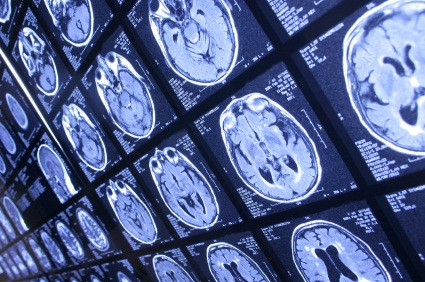
\includegraphics[width=3.5in]{Figure/medical-image-analysis.jpg}
  \end{figure}
  
\end{multicols}
\end{frame}


\subsection{Big Data e Analytics}
\begin{frame}\frametitle{Big Data e Analytics} 

\begin{multicols}{2}

\begin{itemize}
  \item A quantidade de dados digitais está explodindo!
  \item Análise Big Data é estatística com esteroides.
  \item Exemplos: mídia social, compras na internet, notícias, artigos, dados médicos, dados científicos
\end{itemize}

\begin{figure}[hb]
    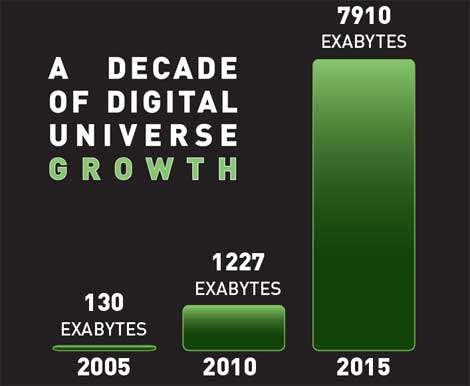
\includegraphics[width=2in]{Figure/digitaluniverse.jpg}
  \end{figure}
  
\end{multicols}
\end{frame}

\end{frame}

\begin{frame}\frametitle{} 
  \begin{figure}[hb]
    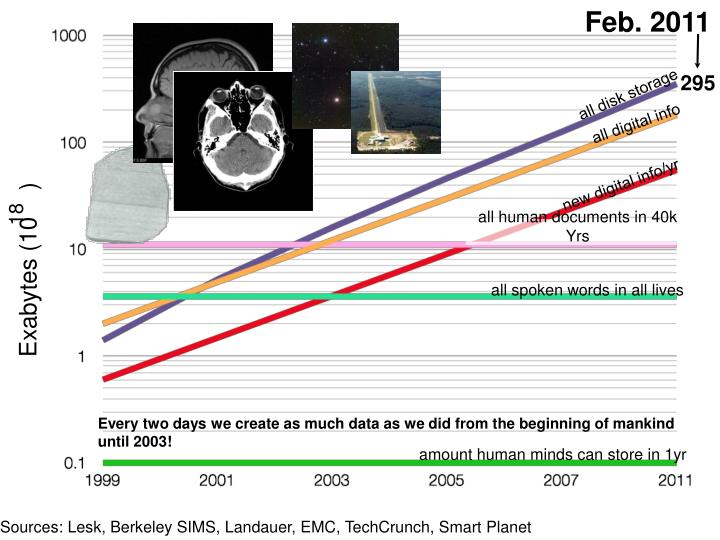
\includegraphics[width=3.5in]{Figure/slide1-n.jpg}
  \end{figure}
\end{frame}

\begin{frame}\frametitle{} 
  \begin{figure}[hb]
    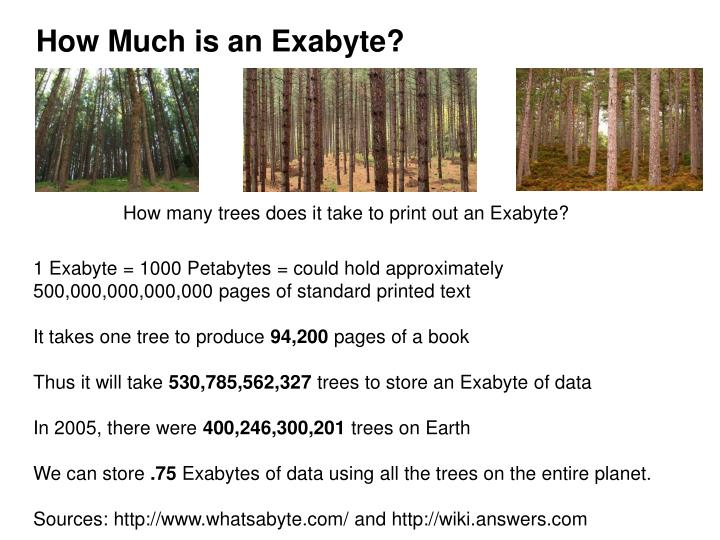
\includegraphics[width=3.5in]{Figure/slide2-n.jpg}
  \end{figure}
\end{frame}

\subsubsection{O Método Científico}

\begin{frame}\frametitle{O Método Científico} 
\begin{multicols}{2}
  \begin{enumerate}
    \item Defina a questão
    \item Observação, pesquisa
    \item Formule uma hipótese
    \item Desenhe e execute um experimento
    \item Analise os resultados
  \end{enumerate}

\begin{figure}[htbp]
    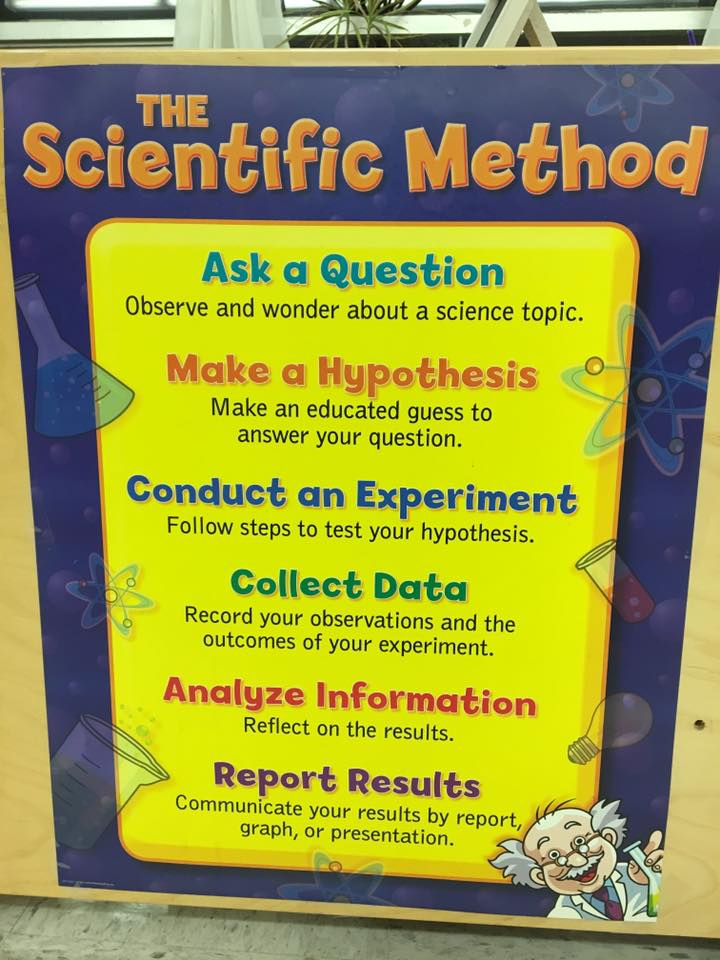
\includegraphics[width=2in]{Figure/thescientificmethod.png}
    \caption{\scriptsize Painel na frente de uma escola de jardim de infância na cidade de Providence, Rhode Island (perto da Brown University).}
\end{figure}
  
\end{multicols}
\end{frame}

\subsection{Evidências}
\subsubsection{Evidências}
\begin{frame}\frametitle{Citação} 
  \begin{figure}[hb]
    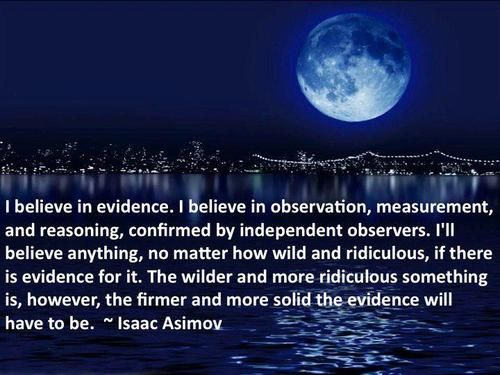
\includegraphics[width=3.5in]{Figure/isaacasimov.jpg}
  \end{figure}
\end{frame}

\subsubsection{Cosmos}
\begin{frame}\frametitle{Cosmos: Episódio 1} 
\begin{figure}[hb]
    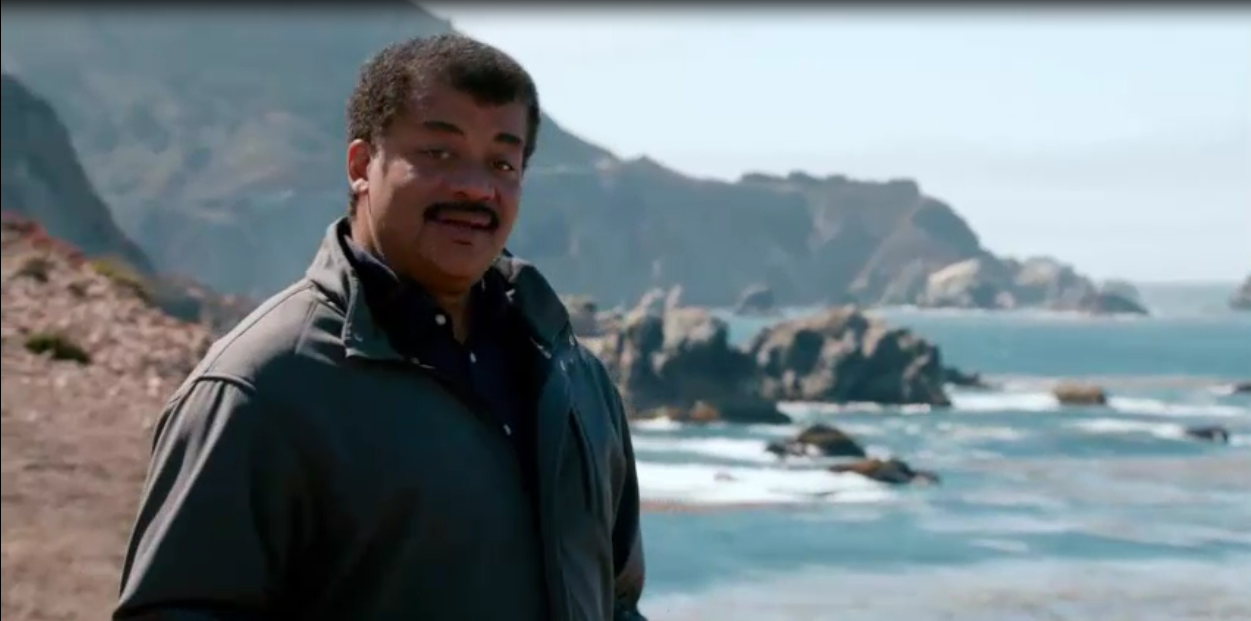
\includegraphics[width=3.5in]{Figure/cosmos1.png}
  \end{figure}
  Assista entre 1:35 e 2:00: \url{https://vimeo.com/153347070}
\end{frame}

%%%
% Aplicação Prática
%%%

% \section{Exemplo Prático}
% 
% \subsection{Turnover de Colaboradores}
% \begin{frame}\frametitle{Turnover de Colaboradores}
% \end{frame}

\end{document}
